\documentclass[10pt]{beamer}
\usepackage[utf8]{inputenc}
\usetheme{default}
\usecolortheme{dove}
\usepackage{textpos}
\usepackage{grid-system}

% \usepackage[rm]{roboto}
\usepackage[T1]{fontenc}
%\usepackage[sfdefault]{roboto}

% po4a: environment frame
% po4a: environment Row
% po4a: environment Cell

\AtBeginSection[] % Do nothing for \section*
{
	\begin{frame}<beamer>
		\frametitle{Übersicht}
		\tableofcontents[currentsection]
	\end{frame}
}

\title{\centering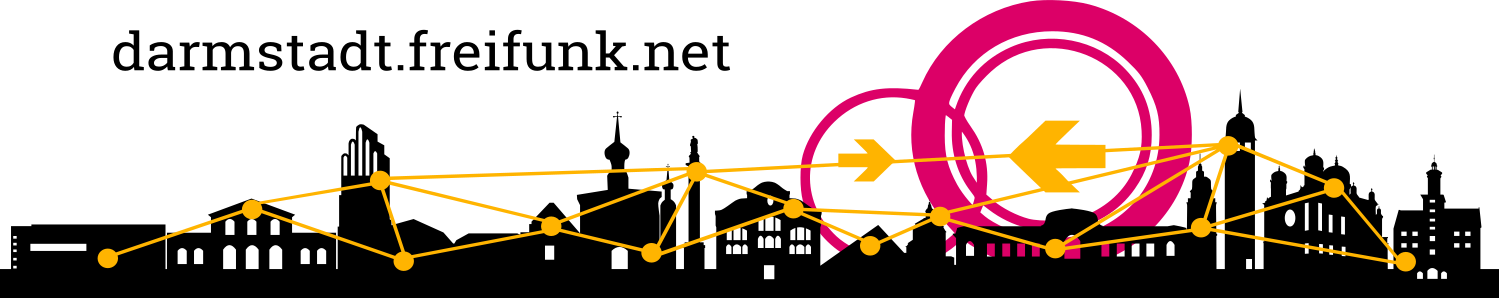
\includegraphics[width=\textwidth]{images/logo-skyline}}
\author{Freifunk Darmstadt,}
\institute[Inst.]{eine Initiative des Chaos Darmstadt e.V.}% würde lieber „ein Projekt des“ schreiben.
\date{\footnotesize 5. November 2015}

\begin{document}


\begin{frame}
\maketitle
\end{frame}

\addtobeamertemplate{frametitle}{}{
\begin{textblock*}{100mm}(0.92\textwidth,-0.5cm)

\includegraphics[height=1cm]{images/logo}
\end{textblock*}}

\begin{frame}{Übersicht}
\tableofcontents
\end{frame}

\section{Was ist Freifunk?}
\begin{frame}
	\frametitle{Was ist Freifunk?}

	\large \textbf{Deutschlandweite Initiative für \emph{freie} (wlan) Netze.}
	\pause
	\vfill
	\centering
	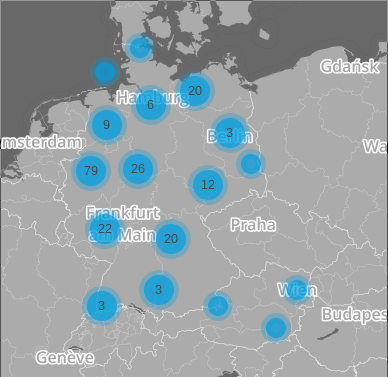
\includegraphics[scale=0.3]{images/2015-10_freifunk-map}
	\itemize{
	\item{über 200 lokale Gruppen}
	\item{bundesweit ca. 20.000 offene Zugangspunkte}
	\item{Teil einer weltweiten Bewegung für offene und freie Netze.}
	}

	
\end{frame}

\begin{frame}
	\frametitle{Wie sieht so ein freies Netz aus?}
	\begin{center}
		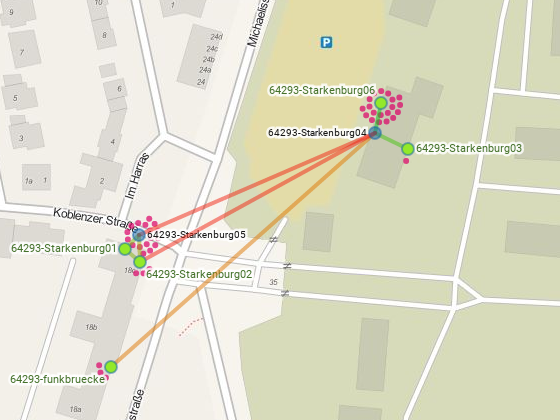
\includegraphics[height=6cm]{images/2015-08-31_starkenburg}
	\end{center}
\end{frame}

\begin{frame}
	\frametitle{Wie sieht so ein freies Netz aus?}
	\begin{center}
		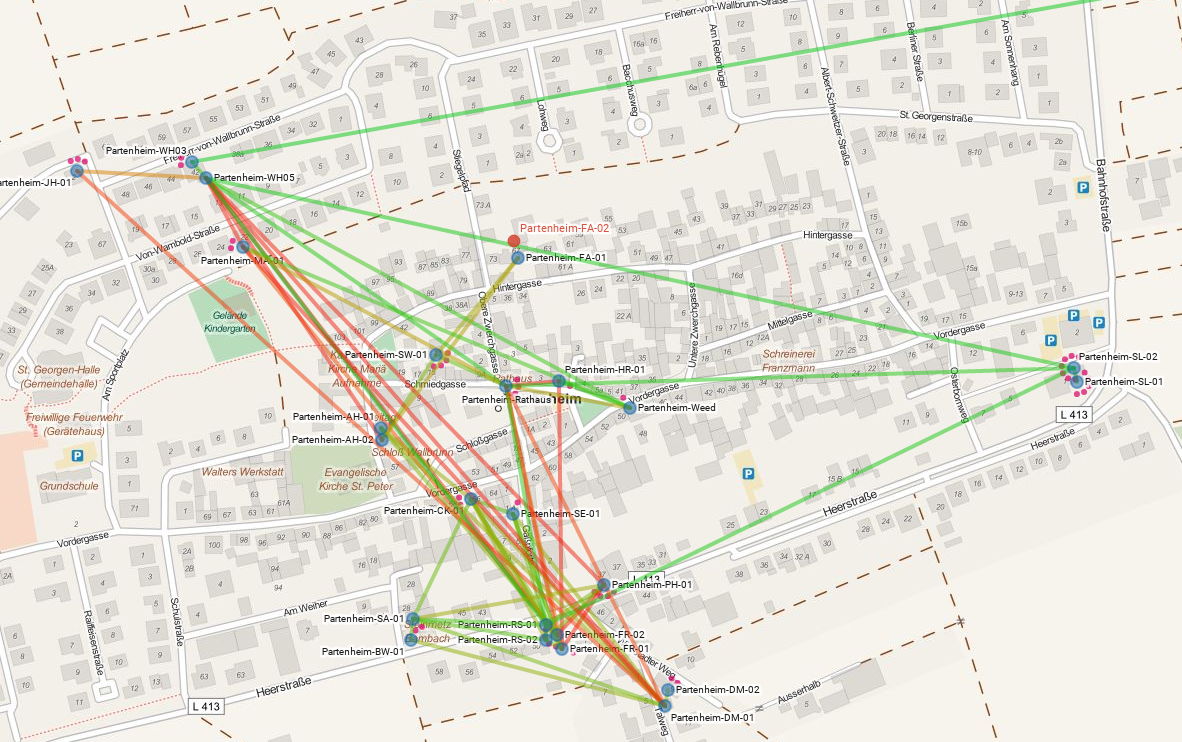
\includegraphics[height=6cm]{images/2015-10_partenheim-map}
	\end{center}
\end{frame}

\begin{frame}{Warum ein freies Netz?}
	\vfill
	\begin{center}
		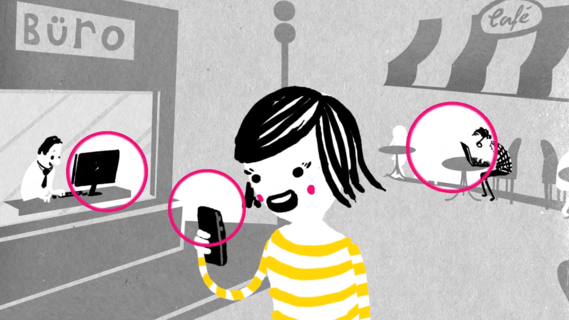
\includegraphics[width=5.5cm]{images/verbindet}
	\end{center}
	
	\begin{itemize}[<+->]
		\item \emph{gleichberechtigt} Netzwerkdienste anbieten und nutzen
		\begin{itemize}
			\item Telefonieren und Chatten
			\item dezentrales Social-Media (z.B Diaspora, Twister)
			\item lizenzfreies Community-Radio
			\item Austausch von Dateien und Medien
			\item lokale Webseiten, Blogsl
			\item \ldots
		\end{itemize}
		\item Internetzugänge \emph{teilen}
		\item \emph{krisensichere} Netzwerktopologie
	\end{itemize}
	\vfill
\end{frame}

\begin{frame}
	\frametitle{Prinzipien}
	\begin{centering}
	\large{\textbf{Wie sollen Kommunikationsnetze beschaffen sein?}}
	\end{centering}
	\pause
	\vfill
	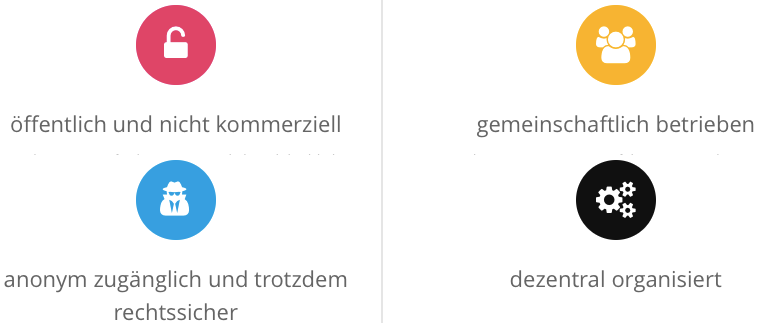
\includegraphics[width=1.1\textheight]{images/principles}$\;$

\end{frame}

\begin{frame}
	\frametitle{Freifunk: offen und öffentlich}
	\begin{columns}[c]
		\begin{column}{5cm}
			
\includegraphics[width=\textwidth]{images/open}
		\end{column}
		\begin{column}{7cm}
			\begin{itemize}[<+->]
				\item freie, ungehinderte Teilnahme an Betrieb und Ausbau des Netzes $\Rightarrow$ Mitmachnetz
				\item Netz im (dezentralen) Besitz der Gemeinschaft
				\item freier Zugang zu Netz und Diensten
				\item keine Unterscheidung nach Ort oder Geldbeutel
				\item \textbf{Unterstützung jederzeit willkommen!}
			\end{itemize}
		\end{column}
	\end{columns}	
\end{frame}



\section{Wie funktioniert Freifunk?}

\begin{frame}{Ohne Freifunk}
	\begin{center}
		%TODO es irgendwie hinbekommen dass die grafiken an einer position beginnen. liegt an dem Text der darunter ist glaube ich.
		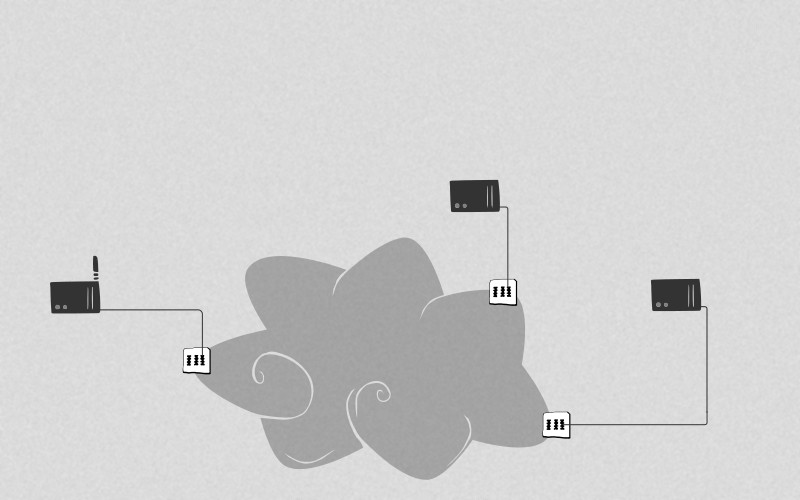
\includegraphics[height=6cm]{images/network_1} \\
		\vfill
		Viele geschlossene (WLAN-)Netze, die nicht miteinander kommunizieren
	\end{center}
\end{frame}

\begin{frame}{Mit Freifunk}
	\begin{center}
		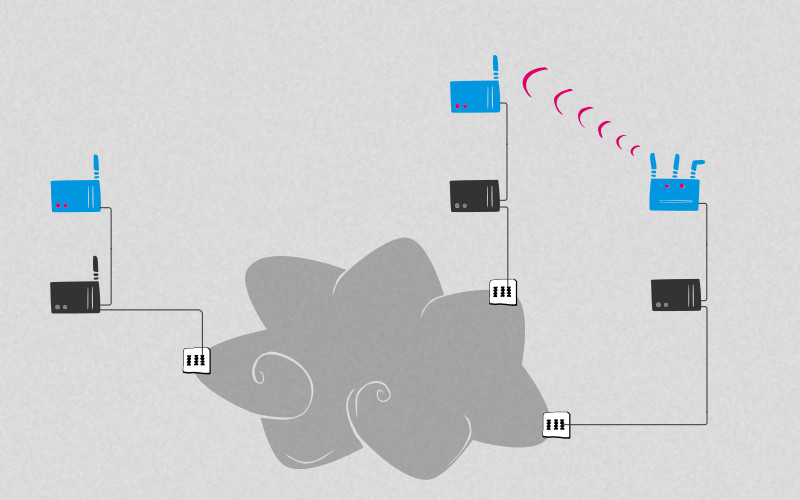
\includegraphics[height=6cm]{images/network_2} \\
		\vfill
		Freifunkknoten bauen ein lokales Netz auf
	\end{center}
\end{frame}

\begin{frame}{Verminderung der digitalen Kluft}
	\begin{center}
		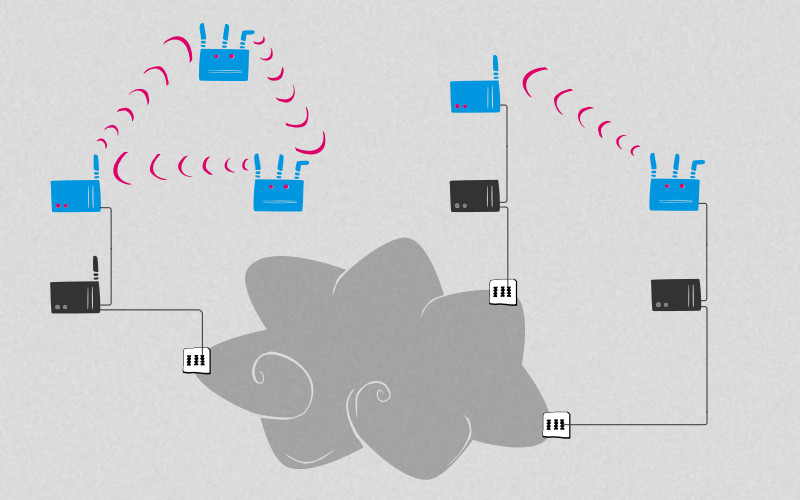
\includegraphics[height=6cm]{images/network_3} \\
		\vfill
		Das Freifunknetz kann mit neuen Knoten erweitert werden,\\ auch dort, wo es keine Internetzugänge gibt
	\end{center}
\end{frame}

\begin{frame}{Das Heimnetz bleibt privat}
	\begin{center}
		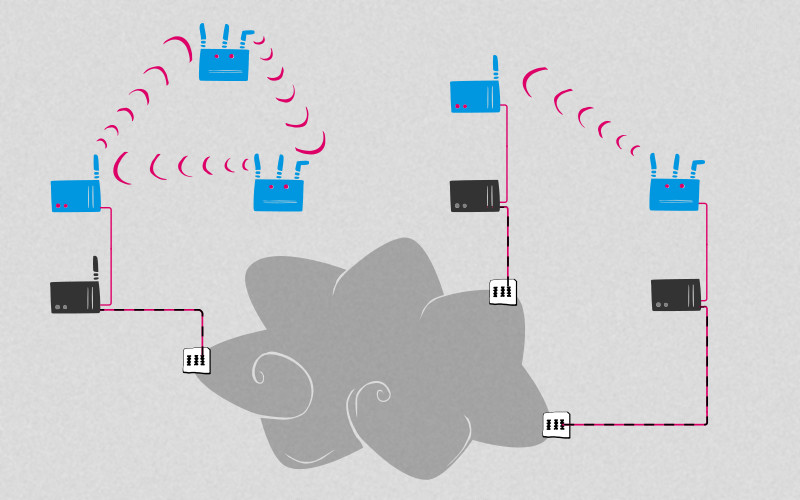
\includegraphics[height=6cm]{images/network_4} \\
		\vfill
		Eigenes Heimnetz und Freifunk-Netz sind getrennt
	\end{center}
	
\end{frame}


\begin{frame}{Zugang zum Internet}
	\begin{center}
		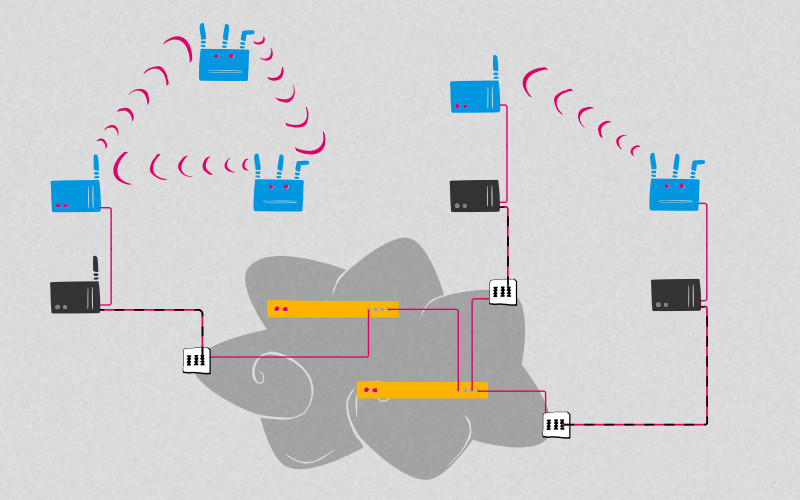
\includegraphics[height=6cm]{images/network_5} \\
		\vfill
		Daten aus dem Freifunknetz werden erst durch unsere Gateways\\ ins Internet weitergeleitet
	\end{center}
\end{frame}


\section{Freifunk in Darmstadt}

\begin{frame}{Stand Oktober 2015}
	\begin{center}
		\vfill
		ca. 240 Knoten, ca. 1000 Clients
		\begin{center}
			\only<1>{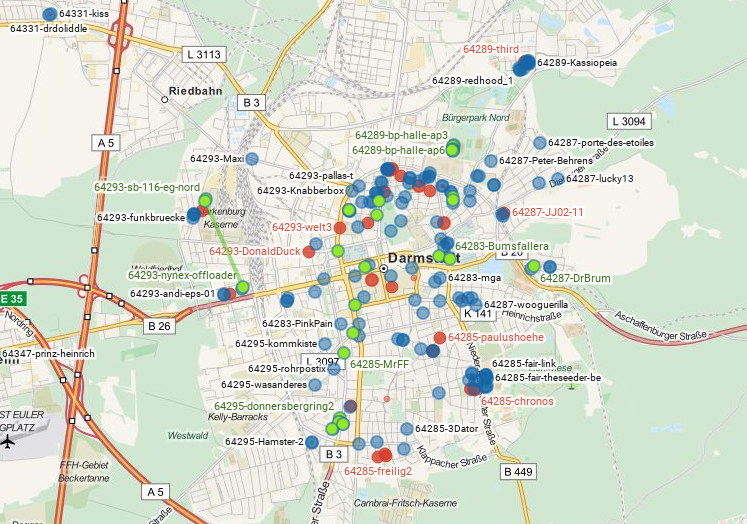
\includegraphics[height=6.5cm]{images/2015-10-03_darmstadt-map}}
			\only<2>{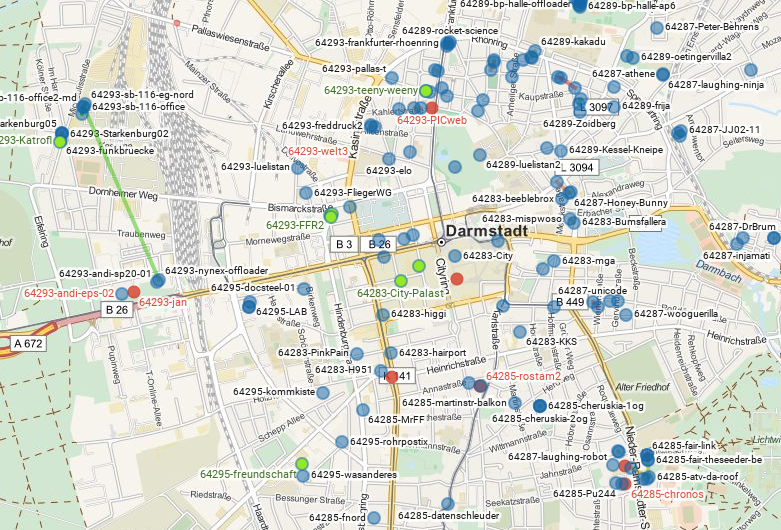
\includegraphics[height=6.5cm]{images/2015-10-30_darmstadt-map}}
		\end{center}
		
		\vfill
		\url{https://map.darmstadt.freifunk.net}
		
		\tiny oder \url{https://map.ffda} im Freifunk-Netz
	\end{center}	
\end{frame}

\begin{frame}{1.x Jahre FFDA-Netz}
	\vfill
	\begin{itemize}[<+->]
		\item 26. Juni 2014: erster Knoten geht online
		\item vor einem Jahr: ca. 30 Knoten
		\item heute: 280 Knoten, davon ca. 220 online
	\end{itemize}
	\begin{center}
		{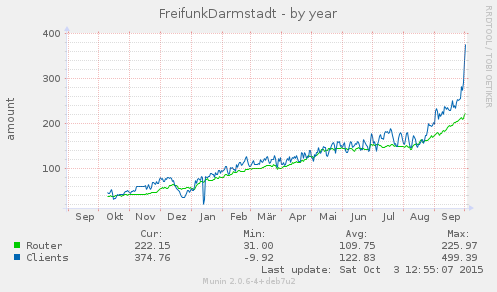
\includegraphics[width=0.8\textwidth]{images/ffda-Okt14-15}}
		%TODO: prepare a graphic showing the refugee client-count explosion with labeled x- and y-axis
	\end{center}
\end{frame}


\begin{frame}{Aktuelle Aufgaben}

	\begin{center}
		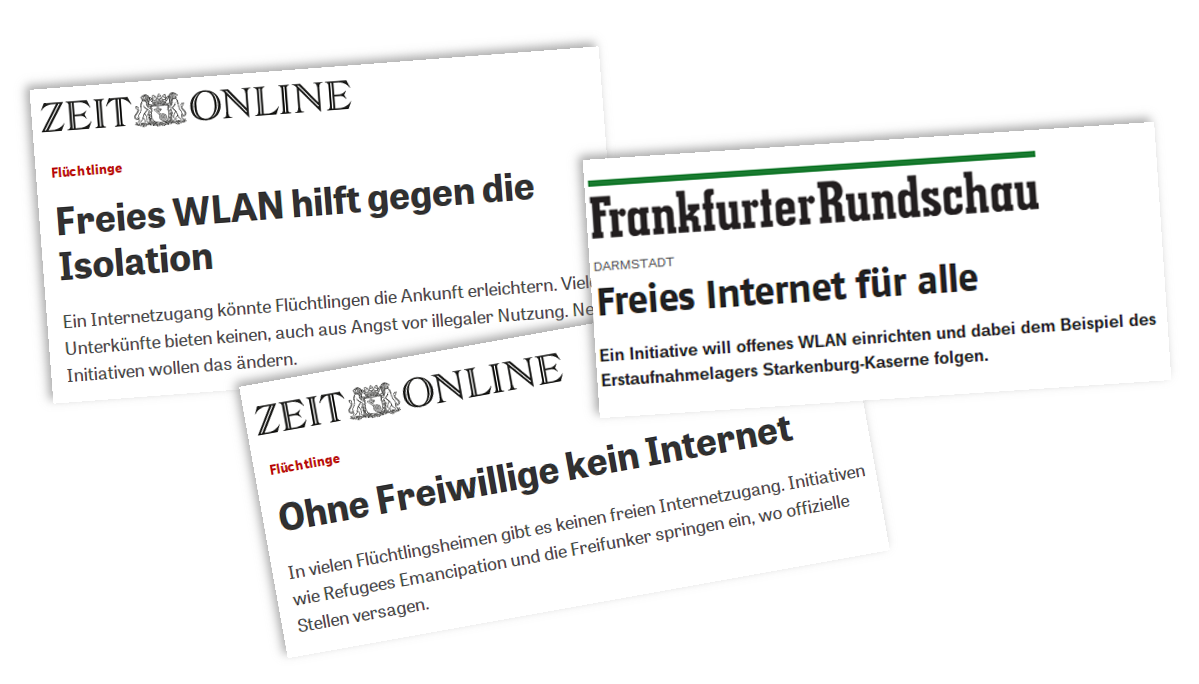
\includegraphics[width=0.7\textwidth]{images/2015-10_presse-fluechtlinge}
	\end{center}
	\begin{itemize}[<+->]
		\item \large Flüchtlingsheime mit Internet versorgen\\
			\tiny auch in Eberstadt, Biebesheim, Stockstadt am Rhein\\
			\tiny hoffentlich bald: Seeheim-Jugenheim, Wixhausen, Mühltal
		\item Öffentlichkeitsarbeit und Community
		\item Netzwerk: Wartung und Ausbau.
	\end{itemize}


\end{frame}


\begin{frame}{Wir freuen uns auf Freiwillige}
	\begin{itemize}
		\item ca. 14 Menschen im Kernteam	
		\item viel Arbeit seit Unterbringung der Flüchtlinge
		\vfill
		\pause
		\item wir treffen uns jeden Montag um 19 Uhr
		\item außerdem online im IRC (\#ffda @ hackint.org)
		\item andere Kontaktmöglichkeiten auf unserer Webseite:\\
		\url{https://darmstadt.freifunk.net/kontakt/}
	\end{itemize}
\end{frame}

\begin{frame}{Q~\&~A $\rightarrow$ Workshop}
\vfill
\centering
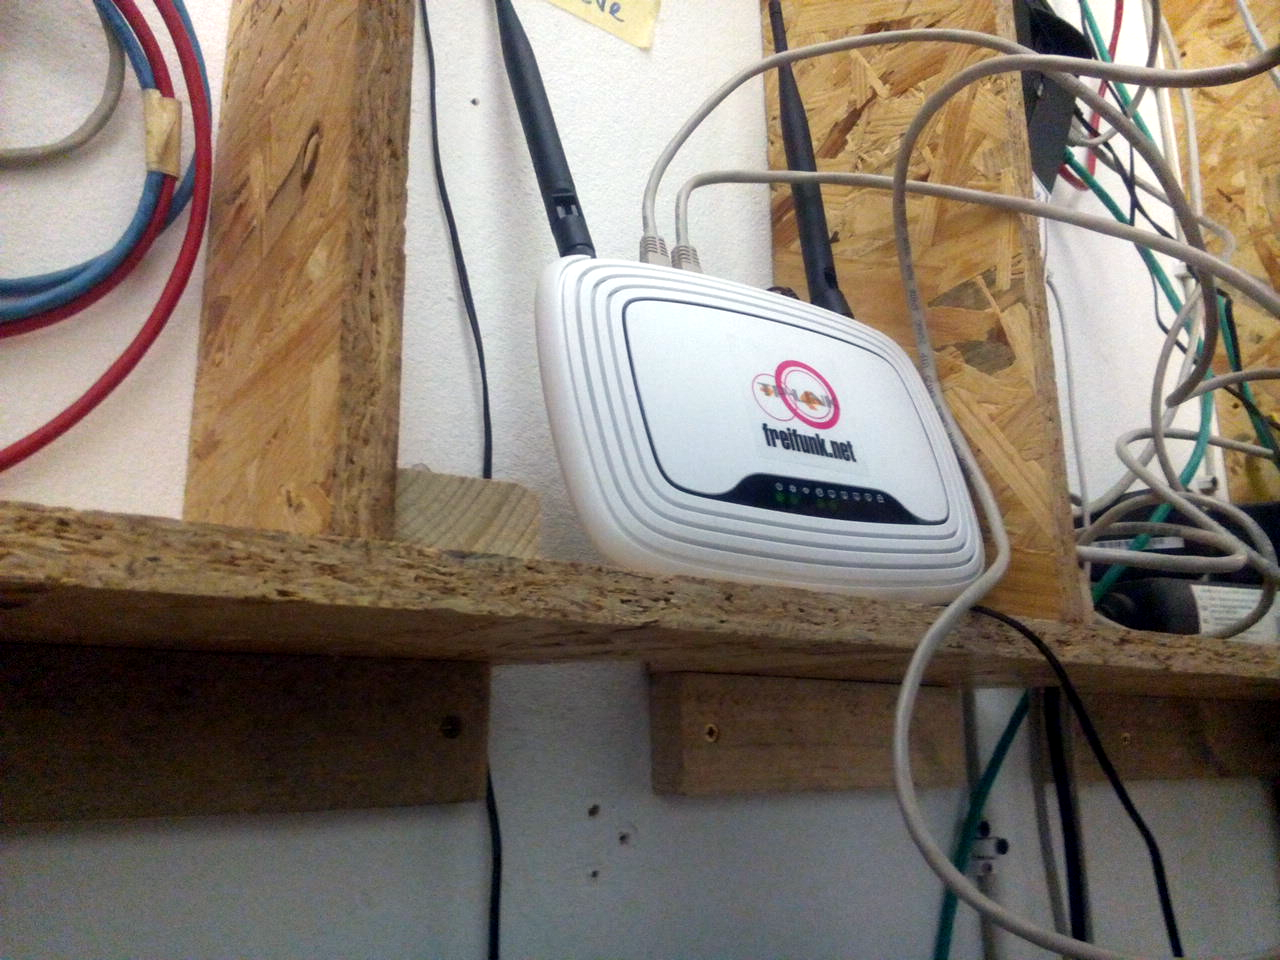
\includegraphics[width=0.7\textwidth]{images/irl_router}
\vfill
\end{frame}

\begin{frame}{Quellen}
\url{https://www.flickr.com/photos/29355306@N06/15613972489/}\\
\url{https://www.flickr.com/photos/yusamoilov/13334048894}\\
\url{https://www.flickr.com/photos/dbaron/2771996590/}
\end{frame}


\end{document}